%!TEX root = ../dokumentation.tex

\chapter{Konzeption}
In den Nachfolgenden Sektionen werden die grundlegenden Technologien und Geräte beschrieben, welche für die Umsetzung dieses Projekts verwendet werden sowie entsprechende Alternativen. Außerdem werden bereits auf dem Markt vorhandene Applikationen mit ähnlichen Funktionsumfang analysiert und deren Stärken und Schwächen herausgearbeitet.\\
Die Analysen beziehen sich hierbei auf die für das Projekt ANNA festgelegten Ziele.

\section{Speech API}
Für die Sprachausgabe sowie vor allem auch für die Spracherkennung, welche zur Interaktion mit der Applikation dienen soll, ist es erforderlich sich mit den zahlreichen vorhandenen Speech APIs auseinander zu setzen, um so die geeignetste für dieses Projekt herauszufiltern.

Der Prozess der Umwandlung des gesprochenen Worts in die geschriebene Form wird als decoding bezeichnet.\\
Die Theorie der Linguistik beschreibt Sprache durch Phonetik, Phonologie, Morphonologie, Syntax, Semantik und Pragmatik. Vor allem die ersten vier dieser Punkte werden von Frameworks zur Umwandlung von Sprache in Text verwendet. Dabei wird versucht das beste Ergebnis durch die Kombination der höchsten Trefferrate der einzelnen Aspekte, durch die Sprache beschrieben wird, zu finden.\\
Die meisten modernen Spracherkennungssysteme nutzen statistische Methoden und maschinelles Lernen zur Verbesserung der von ihnen genutzten Aspekte, welche zur Beschreibung der Sprache verwendet werden.\footcite[vgl.:][]{CMUSphinx} \footcite[vgl.:][S. 410 f]{automaticSpeechRecognition}

In den Nachfolgenden Kapiteln werden insgesamt fünf Speech \ac{API}s untersucht und eine Übersicht über deren Vor- und Nachteile gegeben.

\subsection{Voice Action}
Bei \ac{VA}, welches von Google entwickelt wird, handelt es sich um das standardmäßig mit dem, für mobile Geräte entwickelte Betriebssystem, Android bereitgestelltem Framework zur auditiven Kommunikation zwischen Anwender und System.

Der offensichtlichste Vorteil bei dieser \ac{API} besteht darin, dass sei von Google selbst gepflegt wird und standardmäßig auf Android Geräten verfügbar ist. Da die Applikation so kein eigenes Sprachframework mitliefern muss, wird der Speicherverbrauch entsprechend minimiert.\\
Des Weiteren ergibt sich durch die Verwendung der \ac{VA} \ac{API} die Möglichkeit die eigene Applikation in den Funktionsumfang des von Google bereitgestellten Sprachassistenten ,,Google Now'' zu integrieren. Ein einfaches Beispiel an dieser Stelle wäre eine Wecker-Applikation.\\
Durch die Einbindung von \ac{VA}, wäre es hier möglich, dass die Wecker-Applikation in den Funktionsumfang von Google Now integriert wird, dass wenn ein mit Google Now interagierender Nutzer den Befehl ,,Ok Goole, stelle einen Wecker auf 8 Uhr!'' nutzt, die hier beschriebene Wecker-Applikation von Google Now angesprochen wird um diese Aktion durchzuführen, anstatt den vorinstallierten System-Wecker zu verwenden.\footcite[vgl.:][]{voiceActions}

Der Nachteil bei der Verwendung von \ac{VA} besteht in dem geringen Funktionsumfang für den Entwickler.\\
Dem Entwickler stehen im Wesentlichen nur die Funktionen zur Text in Sprache sowie zur Sprache in Text Umwandlung zur Verfügung. Alle weiteren Verarbeitungsschritte innerhalb dieser Methoden können nicht durch den Entwickler verändert werden um sie so an die jeweiligen Situationen anzupassen.\\
Ein weiterer Nachteil bei der Verwendung von \ac{VA} besteht darin, dass sich die Nutzung auf Android-Geräte begrenzt und es somit nicht möglich ist, es auch für andere Betriebssysteme zu verwenden.\footcite[vgl.:][]{voiceActions}

\ac{VA} bietet für die Berechnung und Umwandlung der Spracheingaben die Möglichkeit die Umwandlung in Text rein auf dem Gerät ausführen zu lassen, jedoch muss dies explizit durch den Nutzer eingestellt werden. Standardmäßig werden die Spracheingaben an Server von Google gesendet um dort verarbeitet zu werden und das Resultat zurück an das entsprechende Gerät gesendet. Zusätzlich wird bei der serverseitigen Verarbeitung eine Kopie der Spracheingabe gespeichert, welche so lange existieren bleibt bis der Nutzer diese eigenständig über eine entsprechende Webseite löscht.\footcite[vgl.:][]{voiceActions}

\subsection{Siri}
Apples Sprachassistent, Siri, bietet seit 2011 die Möglichkeit mit seinem Smartphones und Tablets berührungslos zu interagieren. Allerdings müssen die Geräte ausnahmslos von Apple stammen, um Siri benutzen zu können.\footcite[vgl.:][]{Siriexplained} 

Durch die Entwicklung von Siri weggehend von einem seperaten Modul und hin zu einer stärkeren Intergriergung des Assistenten in das Firmen eigene Betriebssystem, wurde ein großer Fortschritt in Richtung maschineller Unterstützung erzielt. Ab diesem konnte Siri schneller und einfacher mit Apple eigenen Services kommunizieren, welche später noch durch viele weitere externe Services wie Yelp, Rotten Tomatoes, Shazam und einiger anderer online Services ergänzt wurden. Durch die Anbindung all dieser Dienste ist Siri in der Lage noch gezieltere und genauere Antworten auf eingehende Fragen zu geben.\footcite[vgl.:][]{appleSiri} \footcite[vgl.:][]{Siriexplained} 

Dabei hangelt sich Siri an verschiedenen Schritten lang, um das Gesprochene zu erkennen.
Zuerst wird die Stimme in eine kompakte digitale Form umgewandelt. Danach wird ausgewertet, ob der Befehl direkt auf dem Smartphone, also lokal, oder in der Cloud erledigt werden soll. Eingaben wie ,,Spiele einen Song aus meiner Mediathek'' wird lokal ausgeführt. Alle anderen Befehle, welche Zugriff auf das Internet benötigen, werden in der Cloud berechnet. Gleichzeitig wird sowohl lokal auf dem Smartphone als auch auf dem Server das Gesprochene im digitalen Format gegen verschiedenen Statistische Modelle geprüft um herauszufinden, welche Buchstaben benutzt wurden. Derjenige von beiden, welcher eine höhere Wahrscheinlichkeit ausgibt, gibt sein Ergebnis an ein Sprach Modell, welches dann abschätzt welche Wörter gesagt wurden und danach den Befehl ausführen. Wenn sich Siri zu unsicher ist fragt sie jedoch erneut nach.\footcite[vgl.:][]{howSiriWork}

Heute funktioniert Siri mit nahezu allen Apple Produkten, welche ein Mikrofon besitzen. Dennoch schränkt Apple die Benutzung des Services mit nur IOS fähigen Geräten drastisch ein. Dennoch wurde Siri 2016 erstmals für den Zugriff von Drittanbietern Software geöffnet. Wodurch sich Siri erstmals als Assistent für verschiedene Applikationen seit ihrer Entwicklung anbietet.\footcite[vgl.:][]{appleSiri}\footcite[vgl.:][]{Siriexplained}

\subsection{Alexa}
Das Spracherkennungssystem Alexa Voice Services, kurz Alexa, ist der Name der Amazon eigenen Sprachbibliothek, welche in zahlreichen Produkten der Firma verwendet wird. Dabei agiert Alexa als interaktive Kommunikationsschnittstelle zwischen Mensch und Gerät. Inzwischen ist Alexa in der Lage von Haus aus Musik Streaming Dienste anzusprechen, Nachrichten vorzulesen, aktuelle Wetter und Verkehrslagen zu erfahren, Wecker zu stellen, ein Smartes Zuhause zu steuern und die Fragen des Benutzers zu Beantworten.\footcite[vgl.:][]{alexaExplained}

Der Kerngedanke von Alexa ist es Benutzern, Entwicklern und Unternehmen eine Plattform zu schaffen, welche sich einfach durch interne und externe Projekte erweitern lässt. Wodurch die Konfigurierbarkeit bei Alexa im Vordergrund steht. So können Projekte wie ein Smartes Zuhause auch von Endkonsumenten relativ einfach gemeistert werden. Dies ist insbesondere der einfachen Integration eigener Befehle und der offenen Schnittstelle zu verdanken.\footcite[vgl.:][]{alexaDev}

Alexa benutzt wie viele andere Speech \ac{API} Frameworks maschinelles Lernen um sich besser an seine Benutzer anzupassen und eindeutiger Befehle des Gegenüber richtig zu verstehen. Dies beginnt bei der Aufwachwort Erkennung über Antworten bis hin zur Wissens- und Merkmalsextraktion, wobei Amazon in jedem Schritt dem Entwickler Einsicht gewährt.\footcite[vgl.:][]{alexaHow} \footcite[vgl.:][]{alexaDev}

Zusätzlich benötigt Alexa zur Sprachverarbeitung immer eine stabile Internetverbindung, da die tatsächliche Verarbeitung komplett in der Cloud durchgeführt wird. Deshalb gibt es auch immer wieder Kritiker, welche den Datenschutz bei Amazons Sprachbibliothek in Frage stellen, denn um beispielsweise Alexa benutzen zu können muss solange mit gehorcht werden bis das Schlüsselwort ,,Alexa'' fällt.\footcite[vgl.:][]{alexaHow}

Ein beispielhafter Ablauf ist die Aktivierung von Alexa mit Hilfe ihres Aufwachwortes. Danach horcht Alexa auf die Spracheingabe des Benutzers und sendet diese nach Beendigung der Eingabe zum Amazon Alexa Service. Dort angekommen wird die Antwort auf den Amazon Servern gerechnet und zurück an das sendende Gerät geschickt. Auf diesem Gerät wird dann die Nachricht gerendert und dem Benutzer wiederum ausgegeben.\footcite[vgl.:][]{alexaExplained}

Hingegen anderer Speech \ac{API}s horcht Alexa durchgehend auf Benutzereingaben, welches durch die Aufwachworterkennung bedingt ist. Allerdings werden dadurch, gerade in Deutschland, Amazon viele Vorwürfe zum Datenschutz gemacht, das dieser nicht genügend berücksichtigt wird. \footcite[vgl.:][]{alexaDatenschutz}

\subsection{Cloud Speech}
Mit \ac{CS} hat Google einen neuen Dienst zu seiner kostenpflichtigen Cloud Platform hinzugefügt, welcher es ermöglicht Spracheingaben mittels neuronalen Netzwerken in Text umzusetzen. Der Dienst befindet sich aktuell noch in der Betaphase (Stand Januar 2017).

\ac{CS} stellt eine einfach zu verwendende API zur Verfügung, welche es ermöglicht mehr als 80 Sprachen zu erkennen.\\
Die Umwandlung von Sprache in Text erfolgt wie der Name bereits verrät durch das Hochladen der aufgenommenen Spracheingabe und der Verarbeitung in der Cloud. Dabei wird eine Kopie der Sprachaufnahme archiviert.\\
Google verspricht bei der Verwendung von \ac{CS} eine Real-Time Umwandlung der Sprache in Text, indem es nicht wartet bis die ganze Spracheingabe umgewandelt wurde sondern bereits Teilresultate zurückliefert. Durch diese Methodik wird jedoch entsprechend mehr Datenvolumen verbraucht, stellt sich beispielsweise raus das ein bereits zurückgeliefertes Teilresultate nicht korrekt war, was sich aus dem Kontext der weiteren Spracheingabe ergeben kann.

Zusätzlich zur reinen Übergabe von Sprachaufnahmen, bietet die \ac{API} die Möglichkeit zusätzliche Wort Vorschläge welche mitzusenden. Durch diese Vorschläge lässt sich der Kontext der Sprachaufnahme definieren und falsche Ergebnisse vermeiden.\\
Ein Beispiel wäre hier zum Beispiel die Spracheingabe einer Telefonnummer. Da eine Telefonnummer nur aus Zahlen besteht, lässt sich der Kontext entsprechend eingrenzen, so dass bei der Umwandlung keine Wörter sondern nur Zahlen erkannt werden und die Wahrscheinlichkeit der erfolgreichen Umwandlung von Sprache in Text zunimmt.

Durch den Einsatz von Machine Learning und neuronalen Netzen, sowie der stetigen Verbesserung seitens Google, nimmt die Rate der erfolgreichen Sprach in Text Umwandlungen stetig zu.\\
Weiterhin soll \ac{CS} auch die erfolgreiche Umwandlung bei Sprachaufnahmen mit Störgeräuschen ermöglichen.

Der Preis für die Verwendung von \ac{CS} beträgt bei einer Nutzung von Sprachaufnahmen mit einer Dauer von insgesamt 61 bis 1.000.000 Minuten im Monat 0,006\$ pro 15 Sekunden. Sollte die Summe der Längen aller Sprachaufnahmen im Monat unter 61 Minuten bleiben, ist die Verwendung des Dienstes kostenlos (Stand Januar 2017).\footcite[vgl.:][]{cloudSpeechAPI}

\subsection{CMU Sphinx}
\label{sctcmu}
%-ermöglicht definition von grammatik (genauere spracherkennung / kontext bezogen)(sehr Komplex und aufwändig)

\ac{CMU} bietet eine Reihe von Bibliotheken zur Entwicklung von spracherkennungsbasierten Applikationen. Die Bibliotheken stehen hierbei sowohl für Forschungszwecke als auch für kommerzielle Nutzung frei zur Verfügung.

Sphinx bietet die Möglichkeit eigene Sprachmodelle zu entwerfen, Grammatiken zu definieren und die zu erkennenden Wörter kontextuell festzulegen, was die Genauigkeit bei der Umwandlung der Sprache zu Text begünstigt.\\
\ac{CMU} verwendet das Hidden Markov Model, welches in Kapitel \ref{languageProcessing} näher erläutert wird, um das beste Ergebnis bei der Umwandlung einer Spracheingabe hinsichtlich den gegebenen akustischen, lexikalischen und sprachlichen Modellen, zu erzielen.\footcite[vgl.:][]{CMUSphinx}

Durch den kontinuierlichen Entwicklungsprozess welcher 1986 begann, wird die Spracherkennungsgenauigkeit sowie die Geschwindigkeit bei der Umwandlung der Spracheingaben stets verbessert. So ist Sphinx 3, dessen ursprüngliche Verbesserung zu Sphinx 2 in der Genauigkeit der Sprachumwandlung bestand, durch ständige Entwicklungen mittlerweile in der Lage nahezu Echtzeit-Umwandlungen durchzuführen.\\
In Version Sphinx 4 wurde die komplette Sphinx-Engine neu entwickelt und in Java implementiert.

Ein weiter Ableger von Sphinx namens Pocketsphinx wurde speziell Embedded-Systems entwickelt. Diese Version befindet sich aktuell noch in der Entwicklungsphase und ist lediglich als eine Alpha-Version verfügbar (Stand Januar 2017).\footcite[vgl.:][]{wikiCMUSphinx}

Die Umwandlung von Sprache zu Text erfolgt bei Sphinx ausschließlich auf dem Gerät, solange nicht anders durch eigene Backendlösung implementiert.\\
Somit lässt sich der Datenverbrauch bei der Umwandlung von Spracheingaben vermeiden und zusätzlich die Privatsphäre des Anwenders besser schützen, da Sprachaufnahmen nach ihrer Verarbeitung, so lang nicht anders implementiert, gelöscht werden und das Gerät nicht verlassen

\subsection{Vergleich}

In dieser Sektion werden unterschiedliche Speech \ac{API}s in Hinblick auf verschiedene Kriterien miteinander verglichen, um zu entscheiden, welches Spracherkennungssystem für die Applikation genutzt werden soll.

Diese Kriterien sind Konfigurierbarkeit, Verfügbarkeit, Spracherkennung, Abhängigkeit, Lizenz-gebühren, Performance und Entwicklungsstand. Konfigurierbarkeit wurde ausgewählt, da es für die Applikation essentiell wichtig ist eine Schlüsselworterkennung zu benutzen und zusätzlich über die Festlegung von speziellen Sätzen, wie ,,ANNA Spiele den nächsten Song'', die Performance des Systems zu erhöhen. Weiterhin wurde Verfügbarkeit ausgewählt, da viele Speech \ac{API}s eine stabile Internet Verbindung benötigen, um die gesagten Wörter in Text umzuwandeln. Dies führt allerdings zu einer deutlichen Erhöhung des Datenvolumenverbrauchs, wobei diese Umwandlung auch vollständig auf dem Smartphone vollzogen werden könnte. Hinzu kommt, das ähnliche Applikationen zurzeit keine offline fähigen Speech \ac{API}s verwenden, welches ANNA ein Stück weit von existierenden Apps abgrenzen könnte. Das Kriterium Spracherkennung beschreibt den Grad der Zuverlässigkeit des Systems und mit welcher Genauigkeit gesprochene Wörter erkannt werden. Zusätzlich spielt die Abhängigkeit von der \ac{API} vom jeweiligen Betriebssystem eine wichtige Rolle, da nicht alle s\ac{API}s mit jedem Betriebssystem kombiniert werden können. Ein ausschlaggebender Punkt für die User Experience ist die Performance, welche zum einen vom System selbst ausgeht aber zum andern auch deutlich von den Punkten Verfügbarkeit und Konfigurierbarkeit beeinflusst wird. Weiterhin ist der Entwicklungsstand der Speech \ac{API} ausschlaggebend, da Systeme welche noch am Anfang der Entwicklung stehen oder nicht genügend Support erhalten, möglicherweise gewünschte Funktionen noch nicht implementiert haben und Sicherheitslücken aufweisen. Letztendlich spielt die Verwendung der \ac{API} eine große Rolle in diesem Projekt. Einher geht daher auch die Lizenz unter welche diese benutzt werden darf, wie beispielsweise Open Source. 

Im Hinblick auf die Konfigurierbarkeit unterscheiden sich die Speech \ac{API}s maßgeblich. Dies fängt bei keiner Konfigurierbarkeit an und reicht bis zur vollständigen Konfigurierung des Systems. \ac{VA} bietet keinerlei Konfigurationsmöglichkeiten an, lediglich wird die Integration in Google Now angeboten. Bei Siri hingegen werden der Zugriff und die Benutzung des Sprach-Services von Entwicklern erlaubt, jedoch ist es erst seit kurzen verfügbar, wodurch die Entwickler noch limitiert werden. Alexa ist im Gegensatz zu den bisher genannten \ac{API}s ist auf die Entwicklung eigener Services getrimmt, weshalb eine relativ hohe Konfigurierbarkeit angeboten wird. Allerdings wird der Kunde bei der Auswahl des ,,Aufwachwortes'' auf eine kleine Auswahl beschränkt. Im Hinblick auf \ac{CS} flacht der Grad der Konfigurierbarkeit wieder etwa ab, da \ac{CS} zwar eingebunden werden kann, jedoch nicht neue das schreiben neuer Services aus zugelassen wird. Allerdings werden Optionen wie die Übergabe Wortvorschlägen zur Kontextbestimmung angeboten. \ac{CMU} bietet die größte Konfigurierungsmöglichkeit. Dies ist auf den Hintergrund der Speech API zurückzuführen, da sie als Forschungsprojekt entwickelt und für Forschungsprojekte benutzt wird. So können Aplhabete und Grammatiken selber festgelegt werden.\footcite[vgl.:][]{CMUSphinx}\footcite[vgl.:][]{voiceActions}\footcite[vgl.:][]{Siriexplained}\footcite[vgl.:][]{alexaDev}\footcite[vgl.:][]{cloudSpeechAPI}

In Bezug auf Verfügbarkeit grenzen sich die \ac{API}s klar voneinander ab. Weder Siri, noch Alexa oder \ac{CS} sind offline verfügbar. Dies resultiert aus dem Ort der Berechnung. Alle drei genannten Frameworks lassen in der Cloud rechnen, wodurch ein dauerhafter Internetzugang benötigt wird. Siri ist hierbei eine Ausnahme, da auch Spracheinaben auf dem Smartphone direkt gerechnet werden. Dies ist beispielsweise bei Eingaben der Fall, welche keinen Internetzugang voraussetzen. Voice Action hingegen bietet eine komplette offline Sprachsteuerung an, insofern der Nutzer Sprachen abhängige Pakete heruntergeladen hat.
Aufgrund der vollständigen Konfigurierbarkeit dien \ac{CMU} bietet ist auch eine offline Verfügbarkeit möglich.
\footcite[vgl.:][]{howSiriWork}\footcite[vgl.:][]{alexaHow}\footcite[vgl.:][]{cloudSpeechAPI}
Ein essentielles Kriterium für die Qualität der Spracherkennung ist die Genauigkeit mit der die Eingabe extrahiert wird. Dies ist jedoch meist stark von der Umgebung abhängig. Insbesondere weisen ältere PKW einen erhöhten Lärmpegel auf, welcher einer deutliche Erkennung erschwert. \ac{VA} ist von dieser Problematik stark betroffen, da bereits bei einem kleinen Lärmpegel die Genauigkeit drastisch abnimmt. Siri und Alexa arbeiten hingegen mit einem Machine Learning Ansatz, um das gesprochene besser zu verstehen. Hinzu kommt bei Alexa, das bereits Amazon Produkte auch in lauter Umgebung geweckt werden und die Eingabe reagieren können. \ac{CS} arbeitet wie Alexa und Siri auch mit einem Machine Learning Ansatz, jedoch werden hier neuronale Netzen benutzt, womit sich die Genauigkeit über die Zeit immer mehr steigert, da sich das System an die Stimme des Nutzers gewöhnt. Durch die oben genannte Kontext Spezifizierung, welche \ac{CS} anbietet, lässt dich die Genauigkeit der Erkennung weiterhin verbessern. Zusätzlich wird durch gezielte Analyse der Spracheingabe versucht die Störgeräusche heraus zu filtern. Sphinx bietet wie andere \ac{API}s auch die Möglichkeit zur Lärm Unterdrückung an. Die Genauigkeit steigt durch die Mitgabe des Kontextes zusätzlich an.\footcite[vlg.:][S. 7 f.]{alexaHowTo}\footcite[vgl.:][]{howSiriWork}\footcite[vgl.:][]{alexaHow} \footcite[vgl.:][]{cloudSpeechAPI}

Im Hinblick auf die Abhängigkeit von einer Plattform lassen sich die \ac{API}s in zwei verschiedene Gruppen aufteilen. Zum einen die, die Plattform übergreifend genutzt und zum andern die, die Plattform spezifisch genutzt werden können. Dabei schließen sich alle \ac{API}s bis auf Siri Gruppe 1 an. Siri ist in diesem Vergleich die einzige \ac{API}, welche an eine Plattform, IOS, gebunden ist.
\footcite[vgl.:][]{Siriexplained} 

Die Performance der einzelnen Frameworks unterscheidet sich stark durch die verschiedenen Ansätze dahinter. \ac{VA} benötigt relativ lange für das berechnen der Eingabe. Insbesondere dann, wenn das Framework komplett offline genutzt wird. Siri hingegen bietet annähernd Real Time Sprachverarbeitung, durch in der Cloud und lokaler Berechnung, an. Alexa bietet ähnlich wie Siri eine hohe Performance an, jedoch dies nur in der dafür ausgelegten Umgebung, denn Voraussetzung ist eine stabilen Internetverbindung. Mit \ac{CS} lassen sich Realtime Analysen durchführen, jedoch bleibt die Voraussetzung wie bei Alexa gleich. \ac{CMU} ist durch die sehr technische Entwicklung zur nahezu Echtzeit Übersetzung möglich.\footcite[vgl.:][]{howSiriWork}\footcite[vgl.:][S. 3 f.]{sirivsgoogleSpeech}

Der Entwicklungsstand der \ac{API}s ist im Allgemeinen ähnlich. Das bedeutet, dass alle Frameworks stabile Versionen anbieten, jedoch weiterhin in Entwicklung stecken. Dies ist insbesondere bei \ac{VA}, \ac{CS}, Siri und Alexa der Fall, da diese von Firmen vorangetrieben werden. Dies bietet zudem eine gewisse Sicherheit für andere Firmen die diese Frameworks für Projekte benutzen, aufgrund der Tatsache das Google, Apple und Amazon die treibenden Kräfte sind. \ac{CMU} hingegen ist komplett Open Source, wodurch gewisse gefahren bestehen beispielsweise die Einstellung des Supports oder der Weiterentwicklung.

Da die meisten Firmen versuchen mit ihren Produkten Geld zu verdienen müssen fallen häufig Lizenzgebühren an. Dazu zählen die Frameworks Siri, Alexa und \ac{CS}. \ac{VA} hingegen ist für jeden frei zu benutzen. Zusätzlich ist \ac{CMU} als Open Source Bibliothek auch frei zu nutzen. Für die anderen sind jedoch kostenpflichtige Lizenzen, Verwendungsverweise und Bezahlungen nach Volumenverbrauch notwendig.
\footcite[vgl.:][]{CMUSphinx}

Abschließend lässt sich sagen, dass \ac{VA} in Kombination mit \ac{CMU}, das beste Verhältnis aus Komplexität und Leistung bietet. Dies folgt daraus, da sich Siri selbst durch  seine Plattformabhängigkeit ausschließt. Zusätzlich sind sowohl \ac{CS} als auch Alexa momentan noch nicht offline verfügbar, welches die Idee den Datenverkehr auf ein Minimum zu reduzieren nicht untermauern. Daher fällt der Blick auf \ac{CMU} und \ac{VA}. Um bestmögliche Performance und Genauigkeit zu erzielen werden Voice Action und \ac{CMU} in Kombination genutzt. Dabei wird \ac{CMU} für die Spracheingabe und \ac{VA} für die Ausgabe genutzt. Auf der einen Seite bietet \ac{CMU} für die Spracheingabe, Kontextspezifizierung und offline-Verfügbarkeit an, auf der anderen Seite ist für die Ausgabe mit \ac{VA} keine schwerwiegende Konfiguration nötig, da die Ausgabe vom System behandelt wird und zusätzlich die Berechnungen offline ausgeführt werden.


\begin{table}[h]
\centering
\begin{tabular}{ |c|c|c|c|c|c| } 
 \hline
 & Voice Action & Siri & Alexa & Cloud Speech & CMU Sphinx \\
 \hline
 Konfigurierbarkeit & - & N & + & + & ++ \\
 Offline Unterstützung  & ++ & N & - - & - & + \\
 Spracherkennung & N & ++ & ++ & ++ & + \\
 Abhängigkeit & + & - - & + & + & ++ \\
 Lizenzgebühren & + & - - & N & - & ++ \\
 Performance & N & ++ & + & ++ & N\\
 Entwicklungsstand & ++ & ++ & ++ & ++ & N\\
 \hline
\end{tabular}
\par\medskip 
\scriptsize\textbf{Legende:}\begin{labeling}[:]{++}
\item[++] Erfüllt die Anforderung im vollen Maße 
\item[+] Anforderung in größeren Umfang erfüllt
\item[N] Erfüllt die Mindestanforderungen
\item[-] Anforderung in geringen Umfang erfüllt
\item[- -] Anforderung nicht erfüllt
\end{labeling}
\caption{Vergleich Speech APIs}
\label{tabSpeechAPIs}
\end{table}

\newpage
\section{Betriebssystem}
Um die Entwicklungsarbeit für das Projekt nicht unnötig zu vergrößern, wird \ac{ANNA} vorerst nur für ein Betriebssystem entwickelt.\\
Aufgrund der weltweiten Marktanteile fiel die engere Auswahl auf die Betriebssysteme Android und iOS. Andere Betriebssysteme wie Beispielsweise Windows Mobile sind prozentual weltweit gesehen praktisch nicht präsent, da sie zusammen nur einen Anteil von 3\% ausmachen.\footcite[vgl.:][]{androidVSios}

Nachfolgend werden die Betriebssysteme Android und iOS näher Betrachtet und miteinander verglichen. Dieser Vergleich bezieht sich auf die Betriebssystemarchitektur, Marktanteile und Entwicklungsdetails.

\subsection{iOS}
Das Betriebssystem iOS der Firma Apple, hat einen weltweiten Marktanteil von ca. 12\%. Dennoch spielt iOS eine wichtige Rolle in der öffentlichen Wahrnehmung. Dies liegt unter anderem daran, dass iOS ein Jahr vor Android auf den Markt gekommen ist und die Entwicklung von Smartphones somit erheblich vorangetrieben hat. Durch den früheren Marktstart, lag auch die Anzahl der verfügbaren Apps im zugehörigen Appstore weit über der Konkurrenz.\\
Des weiteren legt iOS schon seit Beginn sehr viel Wert auf eine einheitlich, strukturiert und modern erscheinende Benutzeroberfläche.\footcite[vgl.:][]{androidVSios}
Somit wirkt iOS auf viele Smartphone Nutzer als ein sehr benutzerfreundliches Betriebssystem.

iOS und die Hardware auf der es betrieben wird sind stets perfekt aufeinander abgestimmt. Der Grund dafür liegt darin, dass die Entwickler von iOS wissen, auf welchem Endgerät es zum Einsatz kommen wird.

\subsubsection{Architektur}
Nachfolgend wird die in Abbildung \ref{figIOSSystem} sichtbare Architektur von iOS näher beschrieben.

\begin{figure}[h]
	\centering
  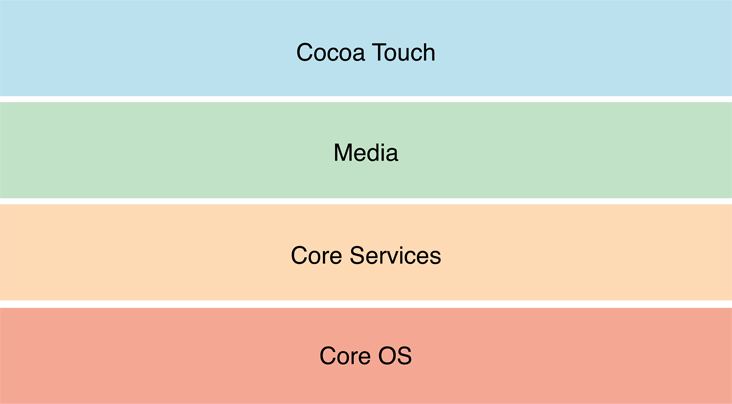
\includegraphics[scale=0.6]{images/iOS_Layers.png}
	\caption{iOS Systemarchitektur (Quelle: \cite[][]{layersOfIos})}
	\label{figIOSSystem}
\end{figure}

Die aus Abbildung \ref{figIOSSystem} ersichtlichen unteren Schichten beinhalten die fundamentalen Dienste. Jede Schicht nutzt die Funktionalitäten der unter ihr liegenden Schicht, um neue anspruchsvollere Dienste zur Verfügung zu stellen.\footcite[vgl.:][]{iOS}\footcite[vlg.:][S. 55 f.]{practicalswift:iosArchitecutre}

Die oberste Schicht, die Cocoa Touch Schicht, bildet mit der von ihr angebotenen Funktionalitäten die Grundlage zur Entwicklung von Applikationen. Bei den hier angebotenen Funktionalitäten handelt es sich um High-Level Features, welche unter anderem App Extensions, Handoff, Document Picker, AirDrop, TextKit, UIKit Dynamics, Multitasking und Auto Layout enthalten.\\
Die Cocoa Touch Schicht bietet somit also die benötigten Funktionalitäten für die Erscheinung sowie der Infrastruktur der Applikation an.\footcite[vgl.:][]{CocoaTouchLayer}

Die zweite Schicht wird als Media Layer bezeichnet und enthält Funktionen für Graphik-, Audio- und Videotechnologien, welche zur Einbindung von Multimediafunktionen in einer Applikation benötigt werden.\footcite[vgl.:][]{MediaLayer}

Auf der dritten Ebene befinden sich die so genannten Core Services.\\
Diese beinhalten fundamentale Systemdienste, welche durch obere Schichten verwendet werden können. Einige dieser Dienste wären beispielsweise Standortsermittlung und Nutzung eines Netzwerks.\\
Diese Dienste werden zum Beispiel für Peer-to-Peer Dienste, die Verwendung des iCloud Speichers sowie SQLite und XML Unterstützung verwendet.\footcite[vgl.:][]{CoreServiceLayer}

Die unterste Schicht bildet das Core OS.\\
Auf dieser Schicht werden low-level Funktionen bereitgestellt, welche für die Verwendung der meisten anderen Technologien benötigt werden.\\
Einige Beispiele wären hier das Bluetooth Framework und das External Accesory Framework, welches es ermöglicht mit Geräten zu kommunizieren, welche an ein iOS-Gerät angeschlossenen sind.\footcite[vgl.:][]{CoreOSLayer}

\subsection{Android}
Android besitzt einen weltweiten Marktanteil von 85\% und wird aktuell von der Open Handset Alliance unter der Leitung von Google weiterentwickelt.\\
Ursprünglich wurde Android von Andy Rubin entwickelt, dessen Unternehmen 2003 von Google aufgekauft wurde.\footcite[vgl.:][]{heiseAndroid}

Nach anfänglichen Startschwierigkeiten hat sich Android heute zum führenden Mobilen Betriebssystem entwickelt. Android wird dabei nicht nur auf Smartphones eingesetzt sondern auch auf Smartwatches, Fernsehern, Tabletts und Autosystemen.\footcite[vgl.:][]{android}

Die rasante Entwicklung von Android und der hohe Gewinn an Marktanteilen ist umso erstaunlicher, betrachtet man das Problem vor dem die Entwickler stehen. Durch die unterschiedlichen Verwendungszwecke von Android und die hohe Anzahl von Geräten unterschiedlicher Hersteller stehen die Entwickler von Android vor der Herausforderung Android stets so zu gestalten, dass es auf selbst ihnen unbekannten Geräten stabil betrieben werden kann.\footcite[vgl.:][]{androidVSios}

\subsubsection{Architektur}
Nachfolgend wird die in Abbildung \ref{figAndroidSystem} sichtbare Architektur von Android näher beschrieben.

\begin{figure}[h]
	\centering
  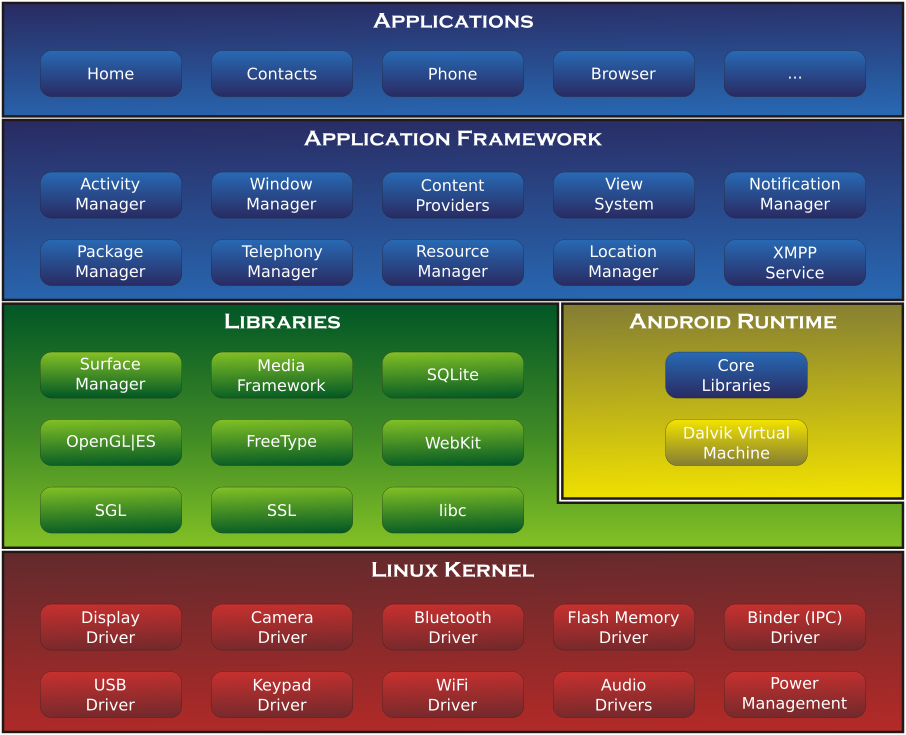
\includegraphics[scale=0.4]{images/Android-System-Architecture.png}
	\caption{Android Systemarchitektur (Quelle: \cite[][]{androidArchitektur})}
	\label{figAndroidSystem}
\end{figure}

Wie aus Abbildung \ref{figAndroidSystem} ersichtlich basiert Android auf einem Linux Kernel. Dieser steuert die Kernfunktionalitäten wie z.B. die Speicher- und Prozessverwaltung als auch das Treibermodell. Der Kernel fungiert somit als Schnittstelle zwischen der restlichen Software und der Hardware des Geräts.\footcite[vgl.:][S. 28 f.]{androidHandbuch}

Die Android Runtime enthält Basisbibliotheken sowie die Dalvik \ac{VM}. Die enthaltenen Basisbibliotheken enthalten die Kernfunktionalitäten der Programmiersprache Java sowie die in C und C++ geschriebenen Komponenten wie beispielsweise OpenGL und OpenSSL.\footcite[vgl.:][S. 9]{einfAndroid} \footcite[vgl.:][S. 27]{androidHandbuch}\footcite[vgl.:][S. 4 f]{braehler:2010}\\
Jede Android Anwendung läuft als eigener Prozess mit eigener Instanz der Dalvik \ac{VM}.\\
Die Dalvik \ac{VM} führt Klassen aus, welche durch einen Java Compiler kompiliert wurden und anschließend in das Dalvik eigene .dex Format, welches besonders speicherschonend ist, transformiert wurden.\footcite[vgl.:][]{androidVSiosArchitekture}\\
Ab Android 5.0 wurde die Dalvik \ac{VM} durch die von Google entwickelte ART Runtime ersetzt. Der Hauptunterschied gegenüber der Dalvik \ac{VM} besteht in der Beschleunigung von Apps und der damit gestiegenen Performance des Systems. Erreicht wird diese Beschleunigung durch eine Ahead-of-Time-Decodierung, bei der Apps bereits bei der Installation übersetzt werden und nicht erst bei der Verwendung wie es bisher unter Verwendung der Dalvik \ac{VM} der Fall war.\footcite[vgl.:][]{artvsdalvik}\footcite[vgl.:][S. 27 f.]{androidHandbuch}

Applikationen für Android werden in Java geschrieben. Android selbst kommt bereits mit einigen Standardapplikationen. Alle von diesen Standardapplikationen verwendeten \ac{API}s die auch für dritte durch das in Graphik \ref{figAndroidSystem} gezeigte Application Framework zur Verfügung gestellt werden. \footcite[vgl.:][S. 10 ff.]{einfAndroid}\footcite[vgl.:][S. 5]{braehler:2010}\\
Die Anwendungsarchitektur ist für eine leichte Wiederverwendbarkeit von Komponenten konizipiert worden. Anwendungen können Komponenten bereitstellen, welche dann wiederum von anderen Anwendungen verwendet werden können.\footcite[vgl.:][]{androidVSiosArchitekture}


\subsection{Vergleich}
Bei der Wahl einer geeigneten Basis für das Projekt \ac{ANNA}, steht vor allem die Erreichbarkeit möglichst vieler Nutzer im Vordergrund.\\
In diesem Punkt liegt Android mit einem Marktanteil von 85\% vor iOS mit einem Marktanteil von 12\%. Die restlichen 3\% teilen sich die weniger verwendeten Betriebssysteme wie beispielsweise Windows Mobile.

Ein weiterer wichtiger Aspekt bei der Wahl des Betriebssystems für \ac{ANNA} besteht im Bereich der Entwicklung des Projekts.\\
Bei der Entwicklung von iOS Applikationen werden die Programmiersprachen Objective-C und Swift verwendet, wohingegen bei der Entwicklung von Android Applikationen die Programmiersprache Java Verwendung findet.\\
Als offizielle Entwicklungsumgebungen werden seitens iOS Xcode verwendet, welches für den Einsatz auf Mac OS konzipiert ist. Für die Entwicklung von Android Applikationen kommt hingegen vorzugsweise die auf IntelliJ basierende Entwicklungsumgebung Android Studio zum Einsatz, die für zahlreiche Betriebssysteme zur Verfügung steht.\\
Beim Entwicklungsprozess spielen auch die durch das Betriebssystem zur Verfügung gestellten Funktionalitäten eine wichtige Rolle.\\
Schränkt das Betriebssystem die Verwendung bestimmter Funktionalitäten zu sehr ein, erschwert dies den Entwicklungsprozess und erfordert mehr Zeit bei der Implementierung geplanter Funktionalitäten des Projekts \ac{ANNA}.

Ein wichtiger Vorteil von iOS gegenüber Android besteht in der nahezu einheitlich verwendeten Betriebssystemversion.\\
Durch die Selbstverantwortlichkeit von Apple für die Verteilung neuer Softwareversionen, besteht hier der Vorteil, dass stets die neuste Betriebssystemversion auf allen unterstützten Geräten installiert wird.\\
Bei Android hingegen sind die einzelnen Gerätehersteller dafür verantwortlich die neuste von Google bereitgestellte Version auf ihren Geräten zu verteilen. Durch diesen Umstand sind eine Vielzahl unterschiedlicher Android Versionen im Einsatz, welche sich auch in ihrem Funktionsumfang unterscheiden. Diese Unterschiede führen bei der Entwicklung dazu, dass nicht alle Android Versionen unterstützt werden können und man so einen Prozentualen Teil der potentiellen Nutzer ausschließen muss.\footcite[vgl.:][]{androidvsiosvergleich}

Um den Entwicklungsprozess durch das Erlernen einer neuen Programmiersprache nicht weiter hinauszuzögern und das Entstehen zusätzlicher Kosten durch fehlende Apple Testgeräte zu vermeiden, fällt die Wahl des Betriebssystems bei diesen Kriterien auf Android.\\
Auch durch die größere Anzahl potentieller Nutzer sowie den große Freiraum bei der Entwicklung, fiel auch bei diesem Kriterium die Wahl auf Android.\\
Trotz der großen Fragmentierung durch die Verbreitung unterschiedlicher Android Versionen, welche unter iOS nicht vorhanden ist, überwiegen die positiven Ergebnisse bei den restlichen Kriterien, so dass als Basis für Projekt \ac{ANNA} das Betriebssystem Android zum Einsatz kommt.

Tabelle \ref{tabAndroidVsIOS} bietet nochmals eine übersichtliche Darstellung der einzelnen Ergebnisse des Vergleichs.
\begin{table}[h]
\centering
\begin{tabular}{ |c|c|c| } 
 \hline
 & iOS & Android \\
 \hline
 Entwicklungssprache & Objective-C/Swift & Java \\
 Entwicklungsumgebung & Xcode & Android Studio  \\
 Zugriff & Limitiert & Nahezu Restriktionsfrei   \\
 Marktanteil &12\% & 85\%\\
 Fragmentierung & gering & hoch\\
 \hline
\end{tabular}
\caption{Vergleich iOS und Android}
\label{tabAndroidVsIOS}
\end{table}

%-beide haben Sicherheitslücken, allerdings werden diese schnell geschlossen

\section{Mikrofon}
\label{chpt:Mic}
In dieser Sektion wird speziell auf die verschiedenen Konfigurationsmöglichkeiten des eingebauten Mikrofons und externer Mikrofone eingegangen, da diese eine gravierende Auswirkung auf die Qualität der Spracheingabe mit sich bringen. Dabei spielen insbesondere die beiden Punkte Position und Design eine große Rolle.

\subsection{Position}
Die Abhängigkeit der Erkennungsrate im Hinblick auf die Position des Smartphones wird besonders deutlich, wenn die Lautstärke im Innenraum des PKW betrachtet wird.
In der Tabelle \ref{tabLautMessungFahrt} sind die Messergebnisse einer Innenraum Schallmessung eines PKW im Straßenverkehr festgehalten.%TODO Fußnote Verwendete App
Dabei ist die durchschnittliche Lautstärke abhängig von der Fahrbahn, dem Wetterverhältnis und der Radioeinstellung. 

Bei einem durchschnittlichen Messwert von 56 dB, welcher im Stand bei laufendem Motor gemessen wurde, ist die Position im Auto nicht ausschlaggebend. Dies bedeutet unabhängig von der Position wurde eine Erkennungsrate von über 90 Prozent erzielt, wobei direkt am Mund die höchste Prozentzahl erreicht wurde. Unter Betrachtung einer durchschnittliche Lautstärke von 80 dB auf der Autobahn resultiert ein deutlicher Einfluss der Sprachqualität. Dies folgt daher, da die Dezibel Skala nicht linear sondern logarithmisch ist. Der Unterschied zwischen einem stehenden Auto (56 dB) und einem fahrenden (80 dB) liegt daher bei dem Faktor 4, welches daraus resultiert, dass 6 dB bereits eine Verdopplung der Lautstärke bewirken. 

Aufgrund dieser Differenz folgt eine große Menge an Störgeräuschen, welche von der Speech APi, \ac{CMU}, herausgefiltert werden müssen, um die Eingaben des Nutzers zu erkennen. Dafür wird im Hinblick auf \ac{CMU} der Spektrale Substraktions Algorithmus verwendet. Unter Verwendung dieses Algorithmus wird trotz erhöhter Umgebungslautstärke eine annehmbare Erkennungsrate erreicht. Zusammen mit der Position kann diese Erkennungsrate sowohl verbessert als auch verschlechtert werden. 

Die verschiedenen Positionen, welche in Bild \ref{figMikroPositionen} zu sehen sind, kombiniert mit unterschiedlichen Smartphones repräsentieren die Erkennungsraten, die in Tabelle \ref{tabErkennungsrate} stehen. Dabei kristallisiert sich heraus, dass die intern verbauten Mikrofone starke Abweichung je nach Smartphone Modell haben. So weist das Mikrofon vom Nexus 5X eine 50 Prozent bessere Erkennungsrate als das LG G2 auf. Gründe für diesen drastischen Unterschied sind das verbaute Mikrofon und die Betriebssystemversion des Smartphones. Zusätzlich lässt sich erkennen, dass zwei der drei Positionen des Smartphones sich von der Erkennungsrate her kaum unterscheiden, jedoch die Position Mittelkonsole eine deutliche Verschlechterung aufweist.
%Lässt sich durch die Grundlegende Wellen Physik beweisen -> Verschlechterung der Qualität. Listing mit Formel Wellenausbreitung in einer Richtung
Dies lässt sich darauf zurückführen, dass die Sprechrichtung des Nutzers nach vorne hin zur Straße gerichtet ist und somit nur eine deutlich verminderte Qualität des gesprochenen in der Mittelkonsole ankommt.

Somit sollte sich das Mikrofon und damit auch das Smartphone unmittelbar vor dem Fahrer des Fahrzeugs oder in einer Halterung in der Nähe des Lenkrads befinden, um eine ideale Qualität der Spracheingaben zu gewährleisten. Zusätzlich empfiehlt sich bei älteren Handy Modellen die Verwendung externe Mikrofone, welches in Sektion \ref{sctAddMic} genauer beschrieben ist. 

\begin{figure}[h]
	\centering
  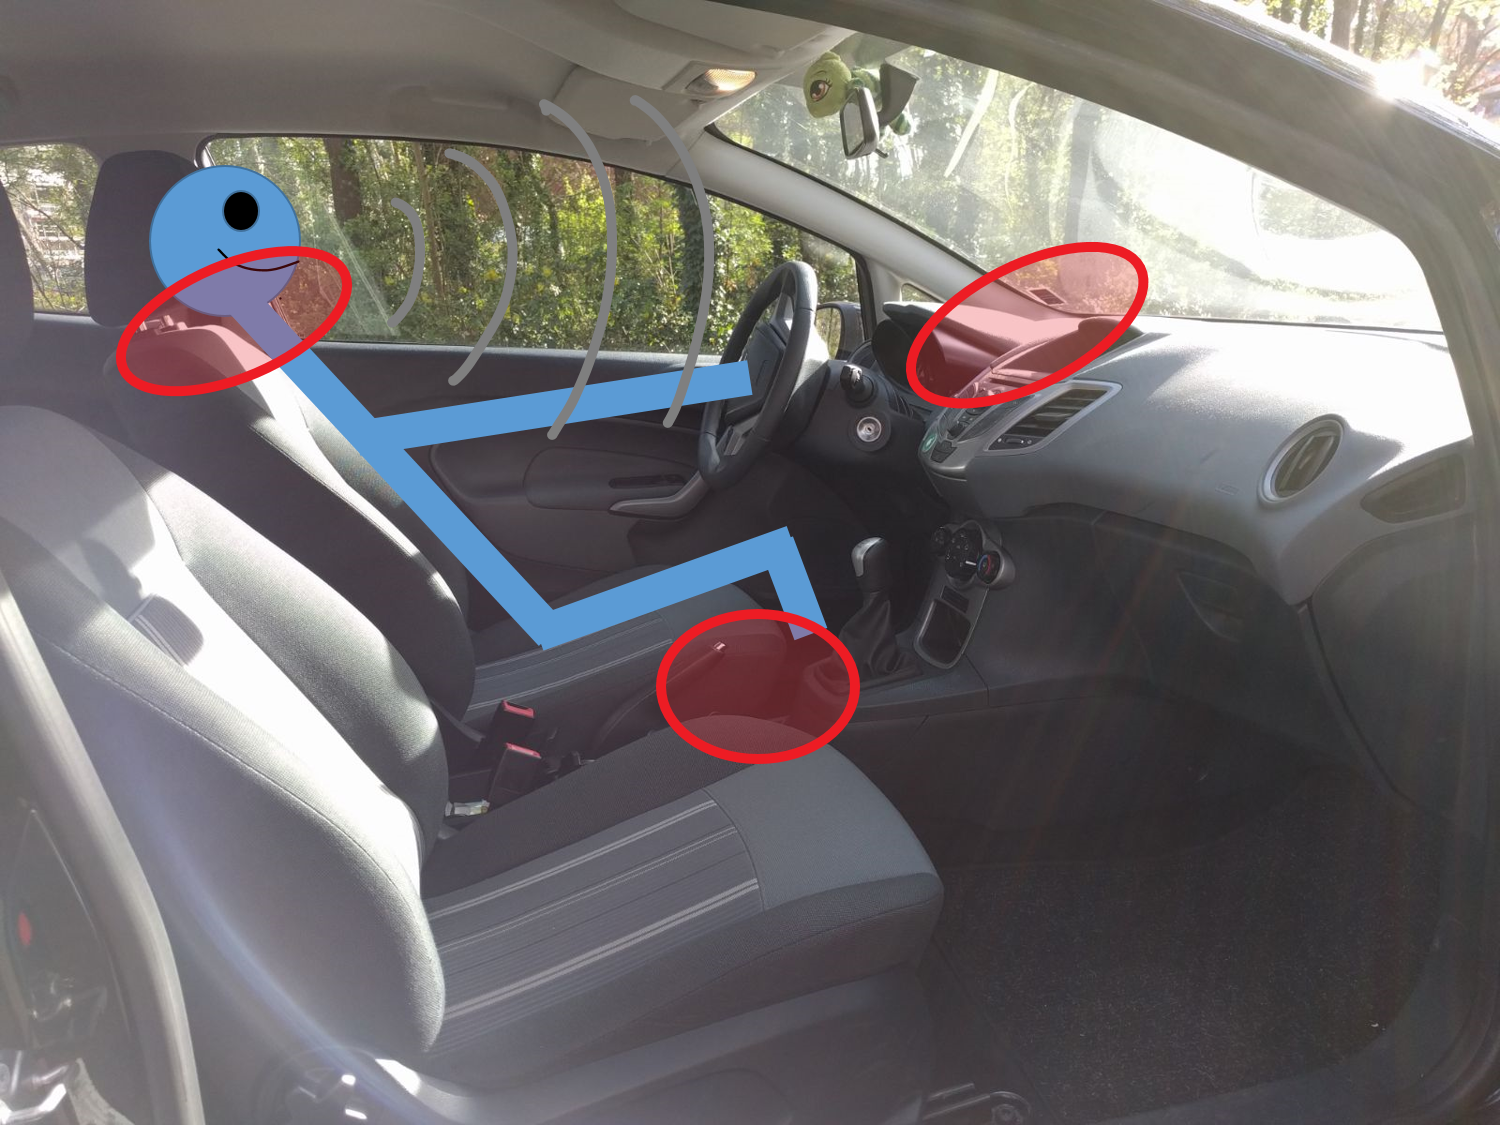
\includegraphics[scale=0.3]{images/position_waves.png}
	\caption{Ford Fiesta Mikrofon Positionen}
	\label{figMikroPositionen}
\end{figure}

\begin{table}[h]
\centering
\begin{tabular}{ |c|c|c|c| } 
 \hline
 Fahrbahn & Wetter & Radioeinstellung & Lautstärkedurchschnitt\\
 \hline
 Autobahn & Regen & Laut & 90dB\\
 Autobahn & Regen & Mittel & 82dB\\
 Autobahn & Regen & Leise & 80dB\\
 Autobahn & Bewölkt & Leise & 77dB\\
 Landstraße & Regen & Laut & 90dB\\
 Landstraße & Regen & Mittel & 81dB\\
 Landstraße & Regen & Leise & 77dB\\
 Landstraße & Bewölkt & Leise & 75dB\\
 Stadt & Bewölkt & Leise & 72dB\\
 \hline
\end{tabular}
\caption{Lautstärkemessung in einem Ford Fiesta Baujahr 2009 }
\label{tabLautMessungFahrt}
\end{table}

\begin{table}[h]
\centering
\begin{tabular}{ |c|c|c|c|c| } 
 \hline
 Smartphone & Mikro & Position & Erkennungsrate & OS Version\\
 \hline
 Nexus 5X & Intern & Am Mund & 95\% & Android 7.1\\
 Nexus 5X & Intern & In Halterung & 90\% & Android 7.1\\
 Nexus 5X & Intern & Mittelkonsole & <10\% & Android 7.1\\
 Nexus 5X & Teufel Move & Am Hals & 98\% & Android 7.1\\
 Nexus 5X & No Name Headset & Am Hals & 88\% & Android 7.1\\

 Samsung S3 & Intern & Am Mund & 92\% & Android 6.1\\
 Samsung S3 & Intern & In Halterung & 88\% & Android 6.1\\
 Samsung S3 & Intern & Mittelkonsole & <5\% & Android 6.1\\
 Samsung S3 & Teufel Move & Am Hals & 95\% & Android 6.1\\
 Samsung S3 & No Name Headset & Am Hals & 85\% & Android 6.1\\

 LG G2 & Intern & Am Mund & 85\% & Android 5.1\\
 LG G2 & Intern & In Halterung & 40\% & Android 5.1\\
 LG G2 & Intern & Mittelkonsole & <5\% & Android 5.1\\
 LG G2 & Teufel Move & Am Hals & 90\% & Android 5.1\\
 LG G2 & No Name Headset & Am Hals & 85\% & Android 5.1\\

 \hline
\end{tabular}
\caption{Erkennungsrate von \ac{ANNA} Sprachbefehlen}
\label{tabErkennungsrate}
\end{table}

\subsection{Design}
%Elektret-Kondensatormikrofone Funktionsweise mit Darstellung
In nahezu allen modernen Konsumergeräte, welche ein Mikrofon verbaut haben, wird das Elektret-Kondensatornmikrofon, auch dauerpolarisierte Kondensatormikrofone genannt, verbaut.
Dieses Mikrofon zeichnet sich durch zahlreiche Vorteile gegenüber anderen Mikrofonarten aus.
\footcite[vlg.:][]{micNutzung}

Die Vorteile resultieren aus dem Aufbau des Mikrofons, welche in Grafik \ref{figElektretMic} zu sehen sind Gegenüber dem normalen Kondensatormikrofon, verwendet das Elektret-Mikrofon als Membran anstatt eines Kondensators eine dauerhaft polarisierte Elektretfolie, wodurch nur der anschließende Feldeffekttransistor zur Verstärkung des Signals mit 1,5 Volt betrieben werden muss. Wohingegen das Kondensator Mikrofon eine dauerhafte Phantomspeisung von 48 Volt benötigt. Aufgrund dieser niedrigen Betriebssppannung, der Kompaktheit und den Herstellungskosten ist das Elektret-Mikrofon in derart vielen Endgeräten verbaut.
\footcite[vlg.:][S. 45 f.]{microphoneBook}

Im Prozess der Tonaufnahme dient das Elektret-Mikrofon als Schallwandler, da es die einfallenden Schallwellen in elektrische Spannungsänderungen transformiert. Die auf die Membran der Elektretkapsel auftreffenden Schallwellen bringen diese zum Schwingen. Die Umwandlung der Schallwellen in elektrisch auswertbare Signale erfolgt durch die Kapazitätsänderung in der Elektretkapsel. Diese lässt sich zeitaufgelöst messen und wird damit zum digitalsierten Abbild der eintreffenden Schallwellen.
\footcite[vlg.:][S. 45 f.]{microphoneBook}\footcite[vlg.:][]{funktionsweiseMic}

\begin{figure}[h]
	\centering
  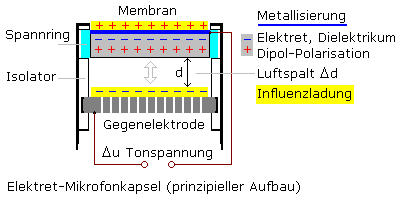
\includegraphics[scale=0.75]{images/aufbau_mic.png}
	\caption{Prinzipieller Aufbau eines Elektret-Mikrofons (Quelle: \cite[][]{funktionsweiseMic})}
	\label{figElektretMic}
\end{figure}


\subsection{Zusätzliches Mikrofon}
\label{sctAddMic}
Aufgrund lauter Umgebungsgeräusche, während der Führung eines Kraftfahrzeuges, fällt die Erkennungsrate je nach Smartphone drastisch ab, welches in Tabelle \ref{tabErkennungsrate} zu sehen ist. Um diesen Fall entgegen zu wirken, empfiehlt sich die Verwendung eines externen Mikrofons. 

Ein externes Mikrofon ist dazu in der Lage, abhängig von seiner Position, die Sprachqualität und somit auch die Erkennungsrate erheblich zu steigern. Als externe können Inear-Headsets, Bluetooth-Headsets aber auch die Freisprecheinrichtung des Autos verwendet werden. Im Rahmen von Testfahrten wurden insbesondere Inear-Headsets getestet. Die Ergebnisse dieser Testfahrten sind in Tabelle \ref{tabErkennungsrate} festgehalten.

Wie der Tabelle zu entnehmen ist wurde sowohl ein Markenheadset, Teufel Move, als auch ein No Name Headset getestet. Unabhängig von der Qualität des Headsets wurde allein durch die Verwendung eines externen Mikrofons eine deutliche Steigerung der Erkennungsrate erreicht, welches sich auf den Abstand zum Mund und die Qualität des Mikrofons zurückführen lässt. Zum Beispiel wurde so eine Steigerung von knapp 50 Prozent in einzelnen Fällen erreicht.

Bei genauerer Betrachtung der beiden Headsets wird lediglich eine minimale Erhöhung der Erkennungsrate deutlich. Auch spielt der Wahl des Smartphones im genaueren des Betriebssystems eine Rolle, da aufgrund des dominierenden Marktanteils von Android, eine deutlich größere Zahl externe Mikrofone zur Verfügung steht.

\subsection{Ergebnis}
Es gibt viele Einflussfaktoren, welche die Sprachqualität und Erkennungsrate der Applikation sowohl positiv als auch negativ beeinflussen können. Die Wichtigsten sind: Position, Typ und Qualität des Mikrofons. Aus unseren Analysen, Testfahrten und physikalischen Grundlagen resultiert die optimale Position des Mikrofones in Höhe der Sprachquelle. Echte Kondensatormikrofone könnten die Erkennungrate weiter verbessern. Wegen des hohen Preises dieser technisch anspruchsvollen Mikrofonvariante scheidet diese für den Masseneinsatz aus.
Abschließend lässt sich feststellen: aktuelle Smartphones liefern wegen der bereits verbauten hochwertigen Komponenten bei guter Positionierung annehmbare Erkennungsraten.  
Bei älteren Smartphones lässt sich die Erkennungsrate bei Einsatz externer Mikrofen auf ein annehmbares Niveau steigern.


\section{Vergleich bestehender Applikationen}
Im Rahmen dieser Sektion wird das Projekt einschließlich der Anforderungen und Ziele mit bestehenden Applikationen verglichen, welche ähnliche Ideen verfolgen. Hinsichtlich dieses Vergleiches wurden die Applikationen Automate-Armaturenbrett und Android Auto ausgewählt. Automate aufgrund der hohen Nutzergruppe und Android Auto, da die Applikation direkt an verschiedenste Google Diensten, beispielsweise Maps oder Hangouts angebunden ist. 
\subsection{Automate}
Automate verfolgt die Idee eines Dashboards für das Auto, damit der Fokus im Auto wieder auf die Straße gelenkt wird. Um dieser Idee gerecht zu werden, sind zahlreiche Funktionen in die Applikation integriert. Dazu zählen das reagieren auf eingehende Nachrichten, das Anrufen von Telefonkontakten, die Navigation von Startpunkt A nach Endpunkt B und die Einbindung des Musikdienstes Spotify und der auf dem Smartphone vorliegenden Musik.
Die integrierten Funktionen spiegeln sich im Layout der Applikation wieder wie in Abbildung \ref{figAutomate} zu sehen ist. Im unteren Teil der Applikation befindet sich verschiedene Icons, welche auf die jeweilige View verweisen. Des Weiteren gibt es eine Overall View, welche in der Abbildung zu sehen ist. Auf dieser View sind wichtige Informationen auf einem Blick zu sehen.
\begin{figure}[h]
	\centering
  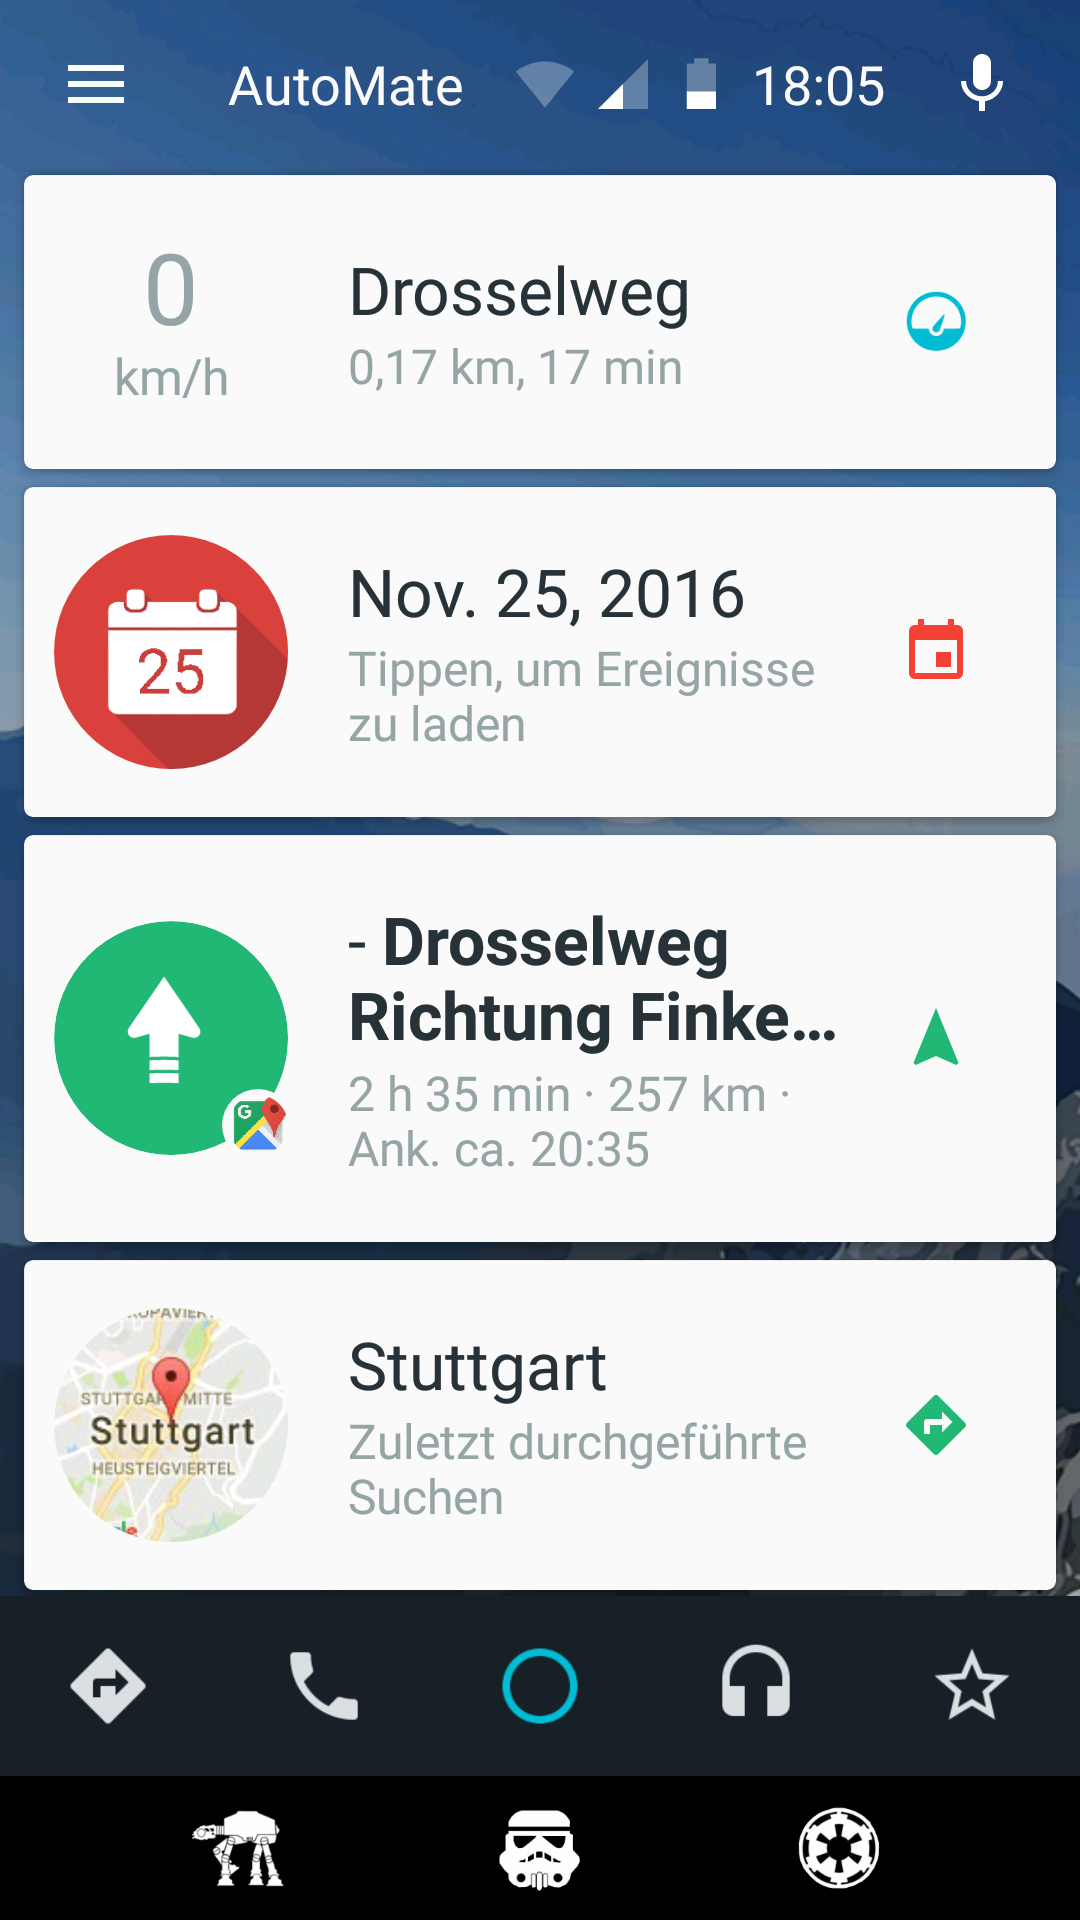
\includegraphics[scale=0.2]{images/Automate_Dashboard.png}
	\caption{Automate Screenshot}
	\label{figAutomate}
\end{figure}
Vergleichbare Strukturen sind auch in den Anforderungen und Zielen dieser Arbeit zu finden. Jedoch wird in Automate eine Modulare Selektierung nicht angeboten. Dies bedeutet, dass dem Benutzer immer alle Funktionalitäten zur Verfügung stehen, auch diese die nicht im Interesse des Benutzers liegen. Im Hinblick auf das Ziel der Applikation, den Fokus auf die Straße zu legen, wird eine Schlüsselwort basierte Aktivierung der Spracherkennung nicht angeboten. Somit ist der Benutzer der Applikation gezwungen, das Mikrofon bei gewünschter Eingabe über einen Knopfdruck zu aktivieren. Die Schlüsselwort Erkennung ist wie in Kapitel \ref{sec:requirements} angesprochen ein Anforderung an das Projekt und in der finalen Applikation enthalten, um eine komplett berührungslose Interaktion nach dem Starten zu schaffen. 

Sowohl Automate als auch \ac{ANNA} sind in der Lage eingehende Nachrichten vorzulesen und auf diese zu antworten. Dies funktioniert bei beiden mit einer Vielzahl von modernen Messengern wie Whats App, Hangouts und Telegram. Allerdings unterscheiden sich die Applikationen in der Spracherkennung. Automate als Sprachinterface Google Now, welches standardmäßig Nachrichten verschicken oder Anrufe tätigen kann. Die Benutzung dieses Interfaces zieht jedoch einen hohen Datenvolumen Verbrauch mit sich, da die Worterkennung auf den Google Servern absolviert wird. Um Ressourcen zu schonen wird bei \ac{ANNA} eine offline fähige Speech \ac{API} namens ,,Voice Action'' benutzt. Dadurch können Sprachkommandos direkt auf dem Smartphone gerechnet werden. 

Eines der Ziele eines Auto Dashboards ist die Navigation, weshalb Automate als auch \ac{ANNA} die Benutzung von Navigationsoftware anbieten. Beispielsweise integrieren beide Applikationen Google Maps als Navigationsservice. Dennoch unterscheiden sich die beiden in der Integrierung des Services. Bei Automate wird beim Eingeben eines Zielortes Google Maps als eigene Applikation gestartet und danach in eine View von Automate geladen. Da Google Maps nicht komplett als eigenständiger Service eingebunden wird, geht sowohl Funktionalität als auch Performance verloren. Im Gegensatz dazu ist Google Maps als eigener Service in \ac{ANNA} eingebaut, wodurch ein kompletter Zugriff auf Funktionalitäten und Performance gewährleistet ist.

Zusammenfassend lässt sich sagen, dass beide Applikationen ihres Zieles gerecht werden, aber sich in ihrer Umsetzung unterscheiden.

\subsection{Android Auto}
Mit Android Auto bietet Google ihren eigenen Auto-Dashboard Applikation an, welche den Google Now Sprachdienst als Basis benutzt. Durch diese Applikation wird der Fokus vom Handy wieder auf die Straße gelenkt, da auch hier die Idee der berührungslosen Interaktion verfolgt wird.
Um diese Idee umzusetzen integriert Android Auto eine Vielzahl an verschiedenen Applikationen, welche über Sprachbefehle gesteuert werden können. Diese decken verschiedene Funktionalitäten wie Navigation, Musik-Streaming und Kommunikation ab, wobei diese Apps größtenteils von Google stammen, zum Beispiel Google Maps, Google Music oder Google Hangouts. Allerdings sind auch externe Kommunikations- sowie Musikdienste, wie beispielsweise WhatsApp, Telegram oder Spotify, eingebunden. 
Dabei spiegelt das User Interface diese Funktionalitäten in mehreren Screens wieder. In Grafik \ref{figAndroidAuto} ist der Aufbau und Verweis auf diese Screens zu sehen, welche sich in einen Home-, Navigation-, Telefon- und Musikscreen unterteilen. Ähnlich wie bei Automate stehen dem Nutzer jederzeit alle Funktionalitäten zur Verfügung, allerdings auch die, die er nicht benötigt.      
\begin{figure}[h]
	\centering
  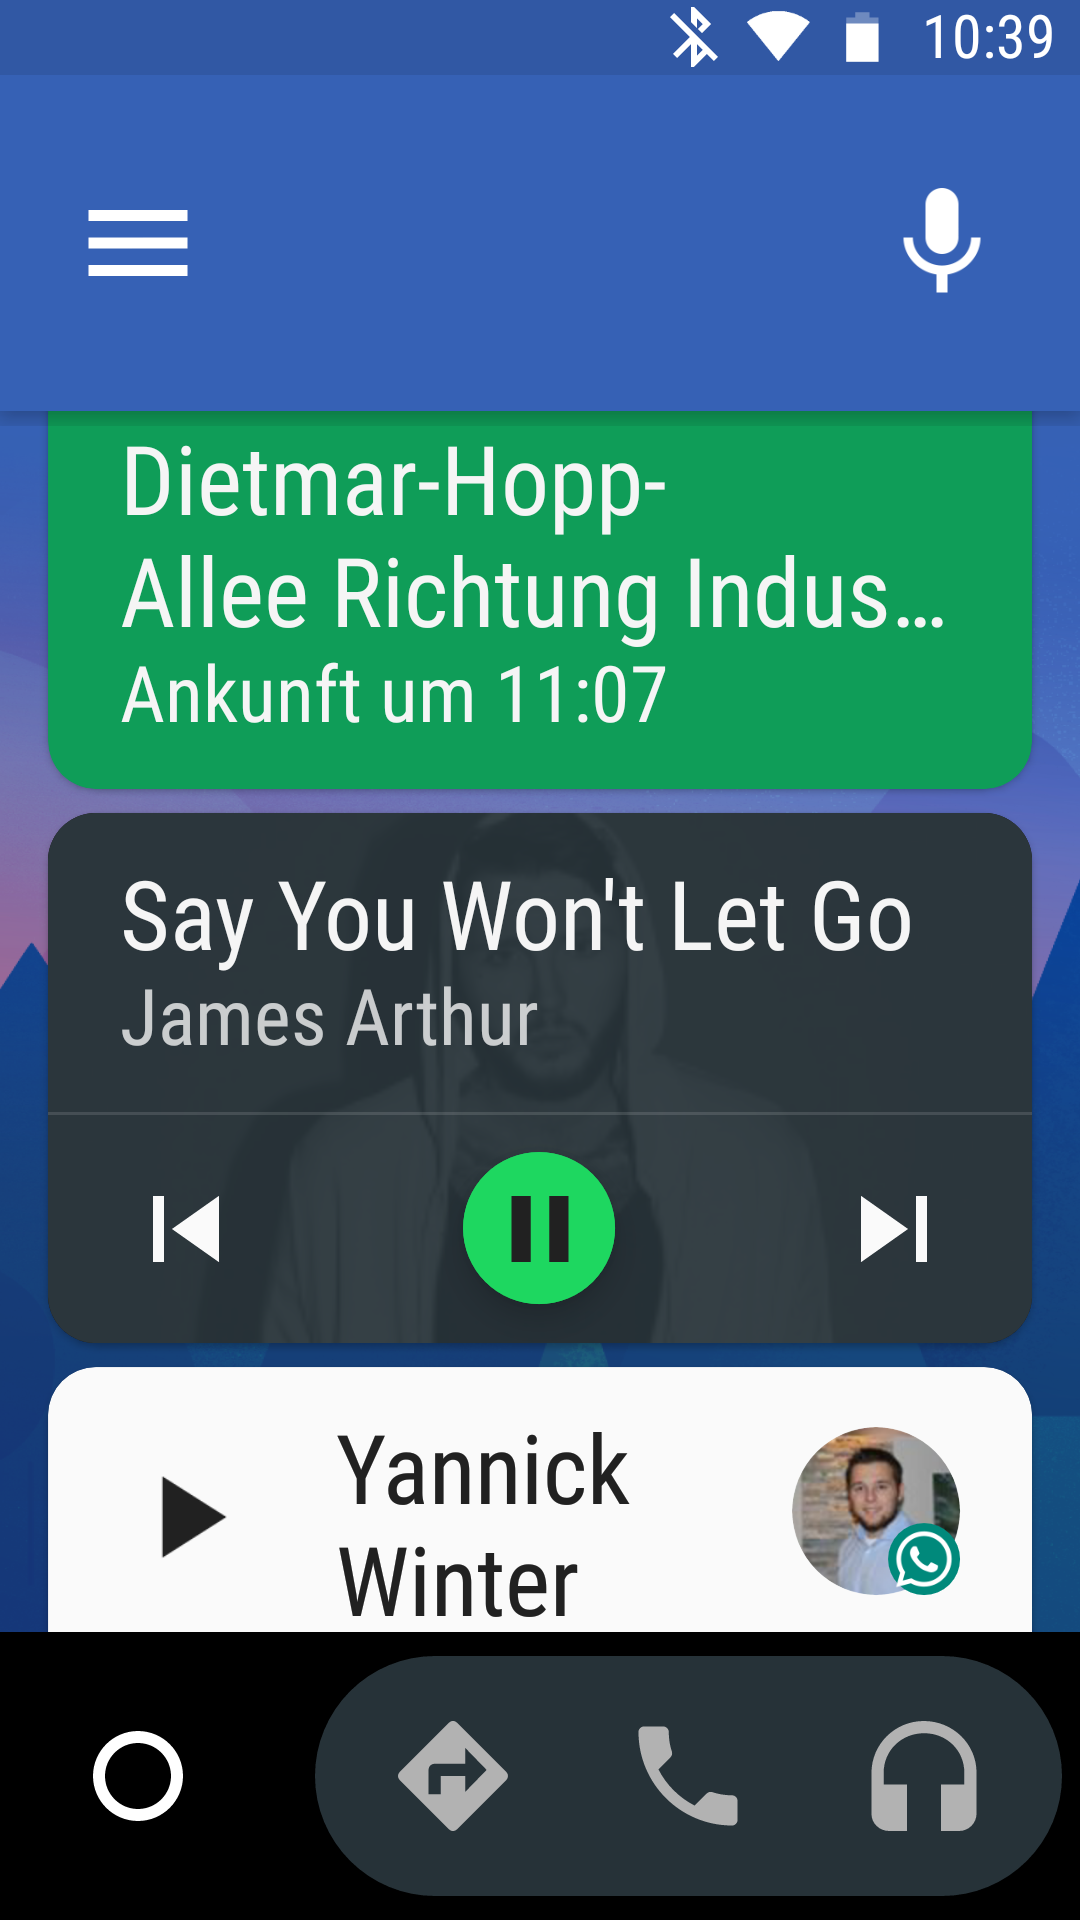
\includegraphics[scale=0.18]{images/Android_Auto.png}
	\caption{Android Auto Screenshot}
	\label{figAndroidAuto}
\end{figure}
Im Hinblick auf die Navigation ist Google strikt und erlaubt als einzigen Dienst das Firmen eigene Google Maps. \ac{ANNA} bietet hier zusätzlich andere Services wie beispielsweise Here Maps.

Android Auto verfolgt als Dashboard Applikation das Ziel der berührungslosen Interaktion, welches mit der Hot Word Erkennung von Google Now im Fundament erreicht wird, bietet jedoch keine weitreichende Steuerung über Spracheingaben an. Befehle, die von Google Now bereits beherrscht werden gezielt umgesetzt. Dies sind zum Beispiel das Versenden von Nachrichten als SMS oder WhatsApp, das Starten einer Navigation oder Anzeigen von Points of Interests auf der Route und das Anrufen von Kontakten. Allerdings erfordern viele weitere, von Android Auto bereitgestellte, Funktionalitäten das Bedienen des Smartphones mit der Hand. Dazu zählen das direkte Antworten auf eingehende Nachrichten und das Steuern von der Musik Dienste. Da diese Funktionalitäten jeder oft genutzt werden und zugleich Kernfunktionen der Applikation darstellen, erzeugen sie wiederum Ablenkungen für den Fahrer, welches dem Gedanken hinter diesem Produkt widerspricht. Im Gegenteil dazu ist es das Ziel im Projekt \ac{ANNA} eine vollständige Kommunikation zwischen Fahrer und Software über Spracheingaben zu schaffen. Wodurch das Fahren des Verkehrsmittels klar im Vordergrund steht. 

Spracheingaben können je nach Konfiguration des Google Dienstes entweder online mit Hilfe von Servern oder offline direkt auf dem Smartphone analysiert und berechnet werden. Wird danach ein Internetzugriff benötigt schickt Google die zuvor berechnete Spracheingabe an die benötigte Applikation oder Service. In diesem Punkt ähneln sich sowohl Android Auto als auch \ac{ANNA}, um in Punkto Zuverlässigkeit den Nutzer zufrieden zu stellen. 

Aus Performance technischer Sicht steht Android Auto gut dar. Dies ist auf die Anbindungsweise der einzelnen Services zurückzuführen. Aufgrund der Tatsache, dass Google die meisten integrierten Services selbst entwickelt hat, kann ein einfacher und schneller Zugriff erfolgen. \ac{ANNA} hingegen benutzt entweder selbst entwickelte oder frei verfügbare \ac{API}s, welche nicht immer vom Entwickler der Services bereitgestellt wurden. Daraus lässt sich meist eine längere Ab- und Anfragezeit ableiten.

Abschließend lässt sich sagen das Android Auto zurzeit relativ wenig Funktionalität anbietet, diese jedoch großenteils gut umsetzt. Jedoch bieten Sprachkontrolle der Applikation und das Einbinden externer Services noch Optimierungspotential.
